

La figure ci-contre représente une pyramide
régulière $SABCD$ à base carrée, de sommet $S$, de hauteur
$SH$. L'unité est le centimètre et on a $SH=6$ et $AD=8$.

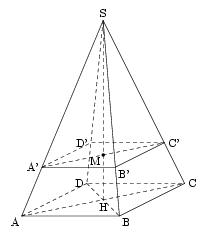
\includegraphics[scale=1]{RepS-45.png} 

\textbf{Première partie}
\begin{enumerate}
\item
\begin{enumerate}
\item Trace, en vraie grandeur, le quadrilatère $ABCD$.
\item Calcule la longueur $AC$ en valeur exacte.
\end{enumerate}
\item
\begin{enumerate}
\item Trace, en vraie grandeur, le triangle $SAH$.
\item Détermine la mesure de l'angle $\widehat{ASH}$ (on donnera un
résultat arrondi au degré près).
\end{enumerate}
\end{enumerate}

%\section{Deuxième partie}
%\begin{myenumerate}
%\item Calcule le volume de la pyramide $SABCD$.
%\item On appelle $M$ le point du segment $[SH]$ tel que
%$SM=\dfrac34SH$. On coupe la pyramide $SABCD$ par un plan
%parallèle à la base et passant par $M$, comme indiqué sur la figure.
%\begin{enumerate}
%\item Quelle est la forme du quadrilatère $A'B'C'D'$ ?
%\item Calcule le volume de la pyramide $SA'B'C'D'$.
%\end{enumerate} 
%\end{enumerate}

